\documentclass{standalone}

\usepackage{tikz}

\begin{document}


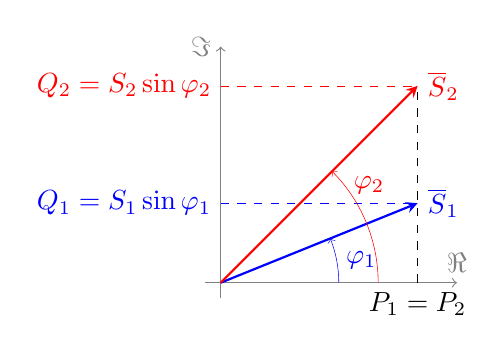
\begin{tikzpicture}
  \draw[->, thin, color=gray] (-0.2,0) -- (3,0) node[above] {$\Re$};
  \draw[->, thin, color=gray] (0,-0.2) -- (0,3) node[left] {$\Im$};
  \draw[-, very thin, dashed,color = black] (2.5, 0) node[below] {$P_1 = P_2$} -- (2.5, 2.5);
  \draw[-, very thin, dashed,color = blue] (0, 1.01) node[left] {$Q_1 = S_1 \sin\varphi_1$} -- (2.5, 1.01);
  \draw [->, very thin, color=blue](1.5,0)  arc[radius = 1.5, start angle= 0, end angle= 22] node [pos=0.5, right] {$\varphi_1$};
  \draw[->, >=stealth, thick, color = blue] (0, 0) -- (2.5, 1.01) node[right] {$\overline{S}_1$};
    \draw[-, very thin, dashed,color = red] (0, 2.5) node[left] {$Q_2 = S_2 \sin\varphi_2$} -- (2.5, 2.5);
  \draw [->, very thin, color=red](2,0)  arc[radius = 2, start angle= 0, end angle= 45] node [pos=0.85, right] {$\varphi_2$};
  \draw[->, >=stealth, thick, color = red] (0, 0) -- (2.5, 2.5) node[right] {$\overline{S}_2$};
\end{tikzpicture}

\end{document}


